\subsection{Spatio-Temporal Self-Attention}
\begin{frame}[allowframebreaks]{Spatio-Temporal Self-Attention}
    \textbf{Spatio-Temporal Self-Attention} extends the Transformer architecture to video data by modeling dependencies across both spatial and temporal dimensions.

    \begin{itemize}
        \item \textbf{Transformers applied to video:} Video frames are treated as sequences, enabling the use of self-attention to capture relationships across space and time.
        \item \textbf{Factorized Attention (e.g., TimeSformer):} Attention is applied separately along spatial and temporal axes, reducing computational cost compared to full spatio-temporal attention.
        \item \textbf{Benefits:} Enables modeling of global context and long-range dependencies in videos.
        \item \textbf{Costs:} Self-attention has quadratic complexity with respect to sequence length, making it computationally expensive for long videos.
    \end{itemize}
\framebreak
    \begin{itemize}
        \item \textbf{Self-Attention Mechanism:} Captures long-range dependencies in both spatial and temporal dimensions.
        \item \textbf{Multi-Head Attention:} Allows the model to focus on different parts of the input sequence simultaneously.
    \end{itemize}
\end{frame}
\begin{frame}[allowframebreaks]{Spatio-Temporal Self-Attention (Nonlocal Block)}
    \begin{figure}
        \centering
        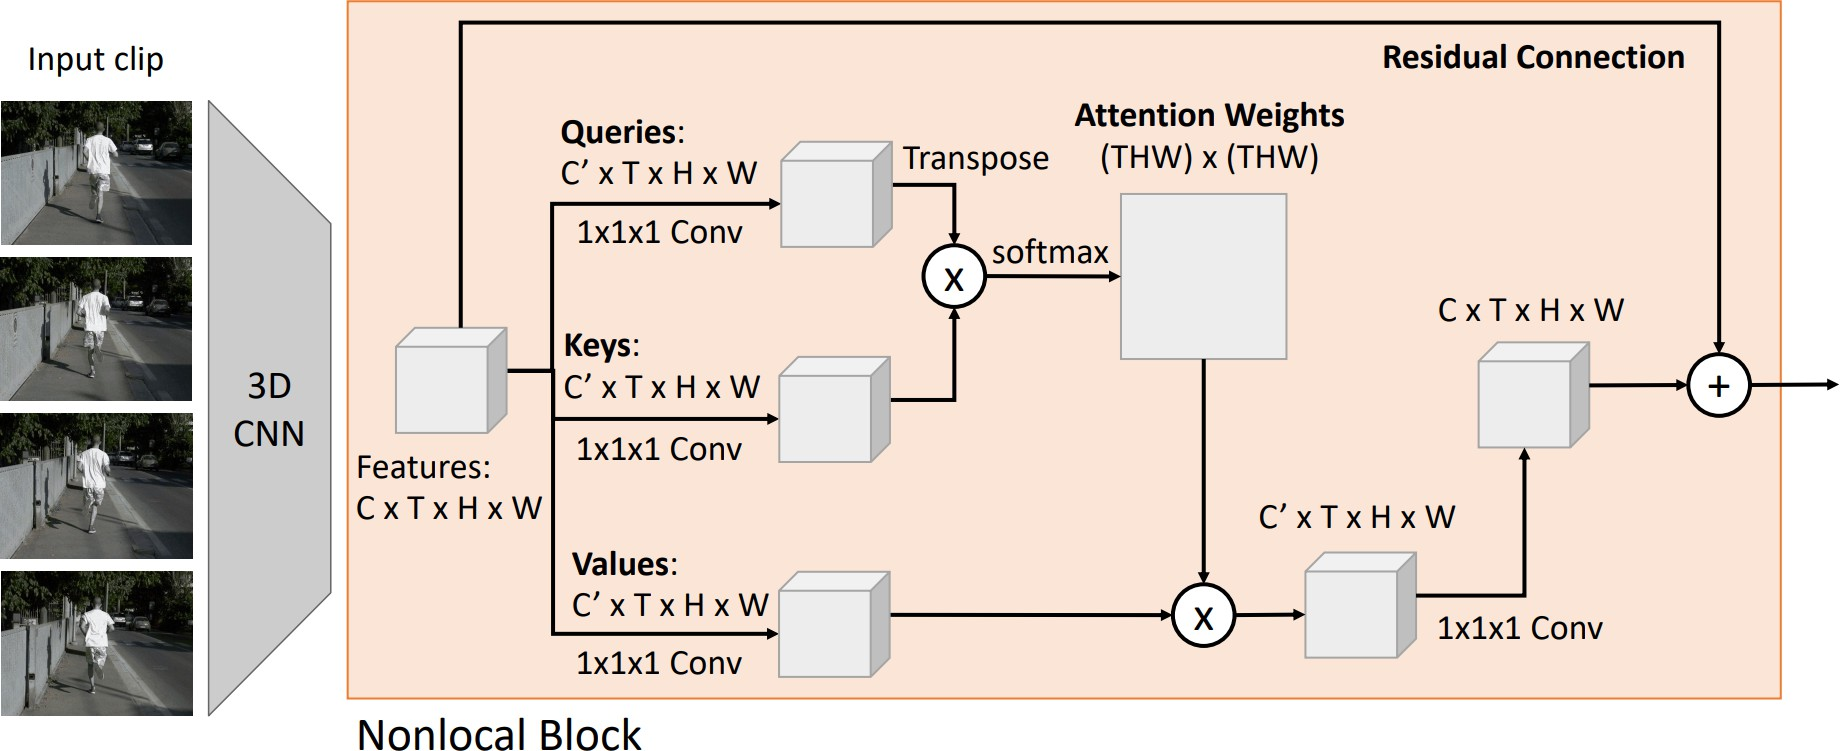
\includegraphics[width=1\textwidth,height=0.9\textheight,keepaspectratio]{images/video/slide_33_1_img.jpg}
    \end{figure}
\framebreak
    \begin{figure}
        \centering
        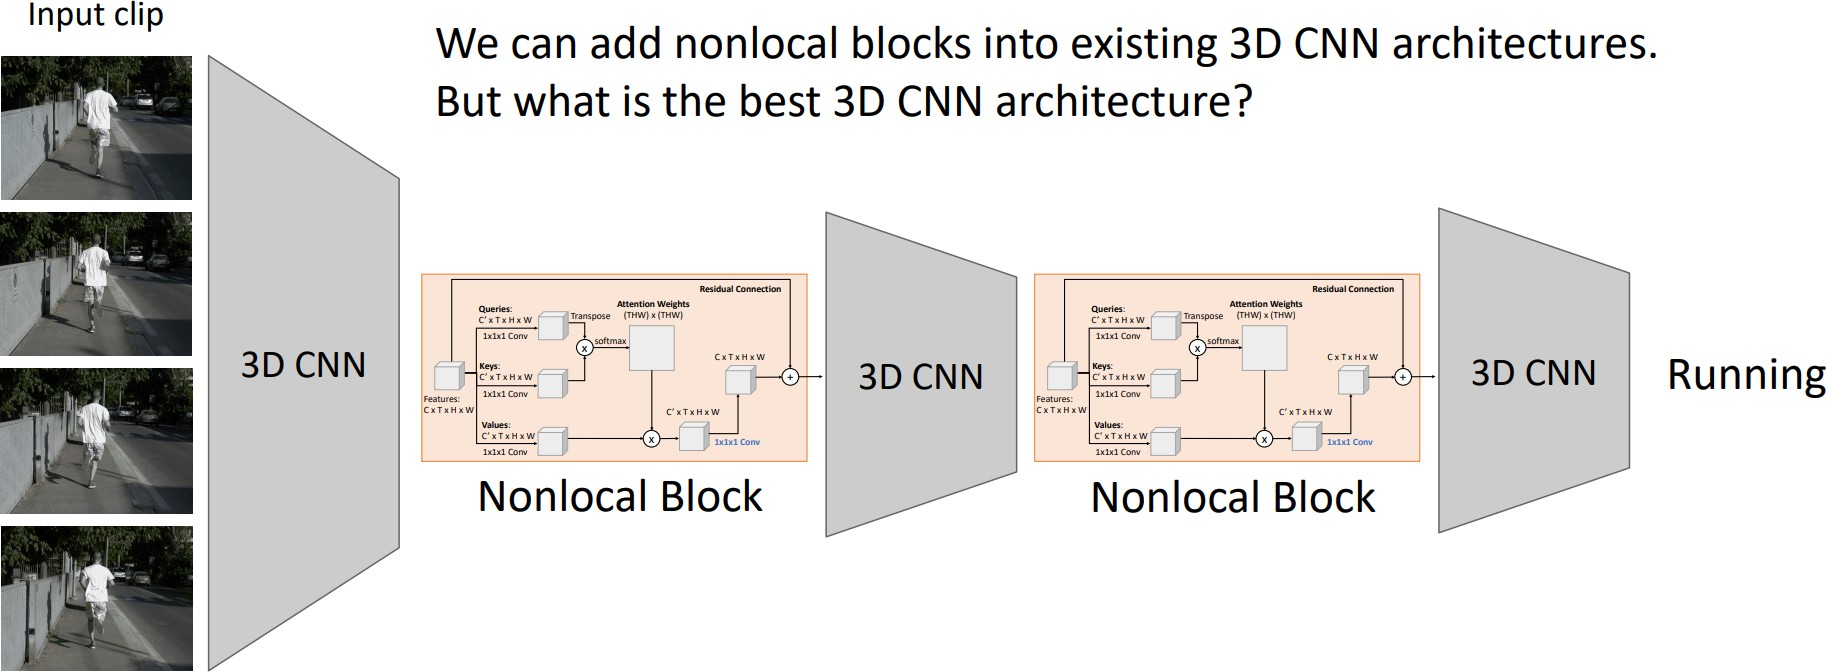
\includegraphics[width=1\textwidth,height=0.9\textheight,keepaspectratio]{images/video/slide_34_1_img.jpg}
    \end{figure}
\end{frame}